\section{Risultati Sperimentali}

I risultati sono ottenuti con la configurazione \texttt{config\_tuned}
($\mu=81$, $p_c=0.675$, $p_m=0.236$, $p_{ls}=0.259$, $\gamma=25$,
$FE=350{,}000$, $R=5$) ottimizzata tramite Optuna.

\subsection{Risultati della Configurazione Tuned}

\begin{table}[H]
\centering
\caption{Risultati HGA --- Configurazione Tuned ($\mu=81$, $k=4$, $e=4$, $\gamma=25$, FE = 350{,}000, R = 5)}
\label{tab:results-tuned}
\footnotesize
\begin{tabular}{@{}lrrrrrr@{}}
\toprule
\textbf{Istanza} & \textbf{Best} & \textbf{Mean} & \textbf{Std} & \textbf{Ottimo} & \textbf{Gap\%} & \textbf{Vei.} \\
\midrule
A-n45-k7     &  1146.77 &  1146.77 &  0.00 &   1{,}146 &  0.07\% &  7 \\
A-n60-k9     &  1355.80 &  1355.80 &  0.00 &   1{,}354 &  0.13\% &  9 \\
A-n80-k10    &  1784.41 &  1785.00 &  0.74 &   1{,}763 &  1.21\% & 10 \\
B-n56-k7     &   712.92 &   712.92 &  0.00 &     707 &  0.84\% &  7 \\
B-n66-k9     &  1326.20 &  1326.56 &  0.44 &   1{,}316 &  0.78\% &  9 \\
B-n78-k10    &  1227.90 &  1228.45 &  0.98 &   1{,}221 &  0.56\% & 10 \\
E-n76-k8     &   740.66 &   741.29 &  1.27 &     735 &  0.77\% &  8 \\
E-n101-k14   &  1090.72 &  1092.38 &  0.83 &   1{,}071 &  1.84\% & 14 \\
P-n50-k10    &   700.66 &   701.37 &  1.42 &     696 &  0.67\% & 10 \\
P-n101-k4    &   691.29 &   691.83 &  0.66 &     681 &  1.51\% &  4 \\
\bottomrule
\end{tabular}
\end{table}

I risultati mostrano un gap medio dello 0.84\%, con picchi di eccellenza
su A-n45-k7 (gap 0.07\%) e A-n60-k9 (gap 0.13\%). La deviazione standard molto
contenuta (spesso $< 1\%$ della media) conferma la robustezza dell'algoritmo.
L'istanza pi\`u difficile si conferma E-n101-k14 (gap 1.84\%) a causa dell'elevato
numero di clienti combinato con un'alta densit\`a di veicoli.

\subsection{Convergenza e Rotte}

\begin{figure}[H]
\centering
\begin{subfigure}[b]{0.49\textwidth}
    \centering
    
\includegraphics[width=\textwidth]{../report/imgs/config_tuned/convergence/convergence_A-n45-k7.png}
    \caption{A-n45-k7 (Set A)}
\end{subfigure}
\hfill
\begin{subfigure}[b]{0.49\textwidth}
    \centering
    
\includegraphics[width=\textwidth]{../report/imgs/config_tuned/convergence/convergence_B-n66-k9.png}
    \caption{B-n66-k9 (Set B)}
\end{subfigure}

\vspace{0.2cm}

\begin{subfigure}[b]{0.49\textwidth}
    \centering
    
\includegraphics[width=\textwidth]{../report/imgs/config_tuned/convergence/convergence_E-n101-k14.png}
    \caption{E-n101-k14 (Set E)}
\end{subfigure}
\hfill
\begin{subfigure}[b]{0.49\textwidth}
    \centering
    
\includegraphics[width=\textwidth]{../report/imgs/config_tuned/convergence/convergence_P-n101-k4.png}
    \caption{P-n101-k4 (Set P)}
\end{subfigure}
\caption{Curve di convergenza per quattro istanze rappresentative --- Configurazione Tuned.}
\label{fig:convergence}
\end{figure}

Le curve mostrano un rapido miglioramento nelle prime 50{,}000--100{,}000 valutazioni,
seguito da un plateau di raffinamento graduale. La convergenza \`e pi\`u rapida
per le istanze di set A e B, mentre per E-n101-k14 e P-n101-k4 l'algoritmo
continua a migliorare fino alle fasi finali.

\begin{figure}[H]
\centering
\begin{subfigure}[b]{0.49\textwidth}
    \centering
    
\includegraphics[width=\textwidth]{../report/imgs/config_tuned/routes/routes_A-n45-k7.png}
    \caption{Rotte per A-n45-k7}
\end{subfigure}
\hfill
\begin{subfigure}[b]{0.49\textwidth}
    \centering
    
\includegraphics[width=\textwidth]{../report/imgs/config_tuned/routes/routes_B-n66-k9.png}
    \caption{Rotte per B-n66-k9}
\end{subfigure}

\vspace{0.2cm}

\begin{subfigure}[b]{0.49\textwidth}
    \centering
    
\includegraphics[width=\textwidth]{../report/imgs/config_tuned/routes/routes_E-n101-k14.png}
    \caption{Rotte per E-n101-k14}
\end{subfigure}
\hfill
\begin{subfigure}[b]{0.49\textwidth}
    \centering
    
\includegraphics[width=\textwidth]{../report/imgs/config_tuned/routes/routes_P-n101-k4.png}
    \caption{Rotte per P-n101-k4}
\end{subfigure}
\caption{Visualizzazione grafica delle rotte finali --- Configurazione Tuned.}
\label{fig:routes}
\end{figure}

Le rotte appaiono logicamente coerenti: i clienti sono raggruppati in cluster
geograficamente compatti, senza incroci evidenti tra i percorsi. L'istanza
P-n101-k4 (solo 4 veicoli per 100 clienti) produce rotte molto lunghe ma
geometricamente ben strutturate.

\subsection{Analisi Statistica}

\begin{figure}[H]
\centering
\begin{subfigure}[b]{0.49\textwidth}
    \centering
    
\includegraphics[width=\textwidth]{../report/imgs/config_tuned/summary/summary_best_vs_bks.png}
    \caption{Costi HGA vs BKS}
\end{subfigure}
\hfill
\begin{subfigure}[b]{0.49\textwidth}
    \centering
    
\includegraphics[width=\textwidth]{../report/imgs/config_tuned/summary/summary_gap.png}
    \caption{Gap percentuale dal BKS}
\end{subfigure}

\vspace{0.2cm}

\begin{subfigure}[b]{0.49\textwidth}
    \centering
    
\includegraphics[width=\textwidth]{../report/imgs/config_tuned/summary/summary_boxplot.png}
    \caption{Distribuzione costi normalizzati}
\end{subfigure}
\hfill
\begin{subfigure}[b]{0.49\textwidth}
    \centering
    
\includegraphics[width=\textwidth]{../report/imgs/config_tuned/summary/summary_runtime.png}
    \caption{Tempo di calcolo vs Dimensione}
\end{subfigure}
\caption{Statistiche globali sulle prestazioni e la stabilit\`a --- Configurazione Tuned.}
\label{fig:summary}
\end{figure}

\begin{figure}[H]
\centering
\begin{subfigure}[b]{0.49\textwidth}
    \centering
    
\includegraphics[width=\textwidth]{../report/imgs/config_tuned/summary/summary_radar.png}
    \caption{Radar Chart per Set}
\end{subfigure}
\hfill
\begin{subfigure}[b]{0.49\textwidth}
    \centering
    
\includegraphics[width=\textwidth]{../report/imgs/config_tuned/summary/summary_generations.png}
    \caption{Generazioni a convergenza}
\end{subfigure}

\vspace{0.2cm}

\begin{subfigure}[b]{0.49\textwidth}
    \centering
    
\includegraphics[width=\textwidth]{../report/imgs/config_tuned/summary/summary_route_length.png}
    \caption{Lunghezza media delle rotte}
\end{subfigure}
\caption{Prestazioni aggregate, convergenza evolutiva e struttura delle rotte.}
\label{fig:summary2}
\end{figure}

\subsection{Confronto tra Varianti di Configurazione}

Per valutare l'impatto dei parametri, la configurazione Tuned \`e stata
confrontata con sei varianti alternative, riassunte in
Tabella~\ref{tab:config-variants}.

\begin{table}[H]
\centering
\caption{Varianti di configurazione a confronto}
\label{tab:config-variants}
\footnotesize
\begin{tabular}{@{}lrrrrr@{}}
\toprule
\textbf{Variante} & $\bm{\mu}$ & $\bm{k}$ & $\bm{e}$ & $\bm{\gamma}$ & \textbf{Generazioni} \\
\midrule
Tuned    &  81 & 4 & 4 & 25 & $\sim$4{,}300 \\
Balanced &  60 & 3 & 4 & 12 & $\sim$5{,}800 \\
Large    & 100 & 4 & 5 & 15 & $\sim$3{,}500 \\
Medium   &  30 & 3 & 3 &  7 & $\sim$11{,}600 \\
Small    &  10 & 2 & 2 &  3 & $\sim$35{,}000 \\
Fast     &   5 & 2 & 1 &  2 & $\sim$70{,}000 \\
\bottomrule
\end{tabular}
\end{table}

La Tabella~\ref{tab:config-comparison} riporta il confronto completo su tutte le
10 istanze.

\input{../../results/table_comparison.txt}

\begin{figure}[H]
    \centering
    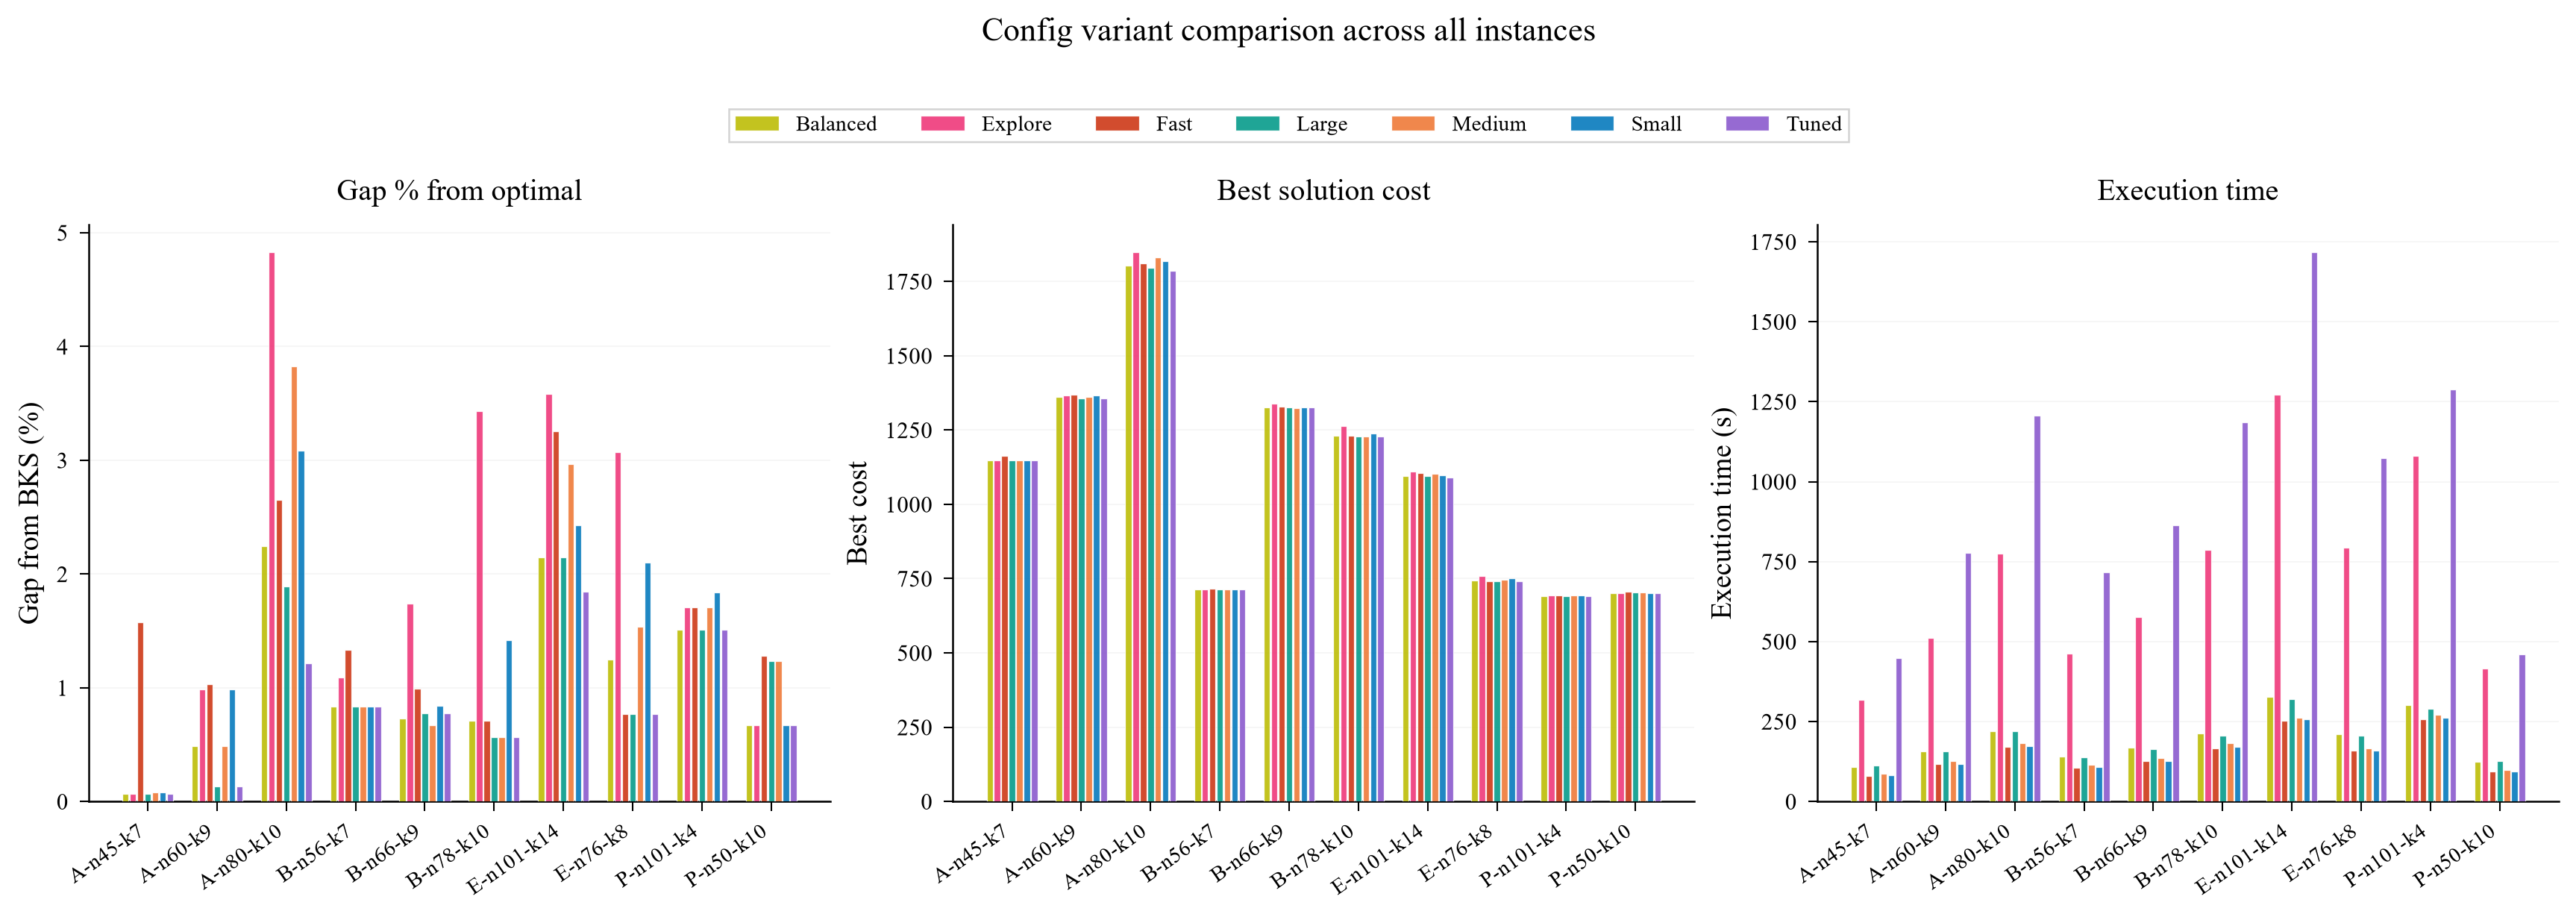
\includegraphics[width=0.8\textwidth]{../report/imgs/summary/summary_config_comparison.png}
    \caption{Confronto visivo tra le sette varianti di configurazione: gap \%,
             costo migliore e tempo di esecuzione.}
    \label{fig:config-comparison}
\end{figure}

\subsection{Discussione}

L'analisi dei risultati permette di trarre diverse osservazioni:
\begin{itemize}[nosep]
    \item \textbf{Qualit\`a}: La configurazione Tuned ($\mu=81$) ottiene un gap medio
    dello 0.84\%. Rispetto a Large ($\mu=100$, gap $\sim$1.0\%), Tuned
    raggiunge prestazioni superiori con una popolazione pi\`u piccola, grazie ai
    parametri calibrati da Optuna ($p_c=0.675$ anzich\'e 0.8, $\gamma=25$
    anzich\'e 15).
    \item \textbf{Effetto della popolazione}: Riducendo $\mu$ da 100 (Large) a 5
    (Fast), il gap medio peggiora progressivamente (Large: $\sim$1.0\%, Fast:
    $\sim$1.7\%). Tuned e Balanced, con popolazioni intermedie (81 e 60),
    rappresentano il miglior compromesso tra diversit\`a genetica e velocit\`a.
    \item \textbf{Robustezza}: La deviazione standard \`e generalmente contenuta
    in tutte le configurazioni ($\sigma < 1$ su 7/10 istanze), indicando
    stabilit\`a intrinseca dell'algoritmo.
    \item \textbf{Trade-off qualit\`a/tempo}: Le configurazioni con popolazione
    minore richiedono pi\`u generazioni ma minor tempo per generazione. Il tempo
    totale \`e dominato dal budget fisso di FE (350{,}000), rendendo i tempi
    comparabili tra tutte le varianti.
\end{itemize}
